%\usepackage[T1]{fontenc}
%\usepackage[utf8]{inputenc}

%!TEX ROOT=../diploma-thesis.tex

\chapter{Implementace prototypů knihoven frameworku}\label{ch:implementace}

%\goal{Uveden\'{\i} kapitoly a nast\'{\i}něn\'{\i} obsahu}
Součást\'{\i} zadán\'{\i} této práce je implementace prototypů
knihoven frameworku navrženého v kapitole~\ref{ch:navrh}
pro tři rozd\'{\i}lné platformy, z nichž jedna mus\'{\i} b\'yt \textit{Java}.
Tato kapitola popisuje výběr plaforem a konkrétní implementace
knihoven pro tyto platformy. Jelikož jednotlivé implementace
vycházejí ze stejného návrhu, kompletní implementace
je popsána pouze pro platformu Java. Ostatní implementace jsou
shrnuty komparativní metodou. Součástí kapitoly je i stručný popis
použitých technologií.

\section{V\'yběr použit\'ych platforem}

%\goal{Jaké jsme vybrali dalš\'{\i} platformy a proč}
Mimo jazyk Java, kter\'y byl určen zadán\'{\i}m, byla pro
implementaci vybrána platforma jazyka \textit{Python} a platforma \textit{Node.js},
která slouž\'{\i} jako běhové prostřed\'{\i} pro jazyk \textit{JavaScript}.
V\'yběr byl proveden na základě aktuáln\'{\i}ch trendů ve světě softwarového
inžen\'yrstv\'{\i}~\cite{githut}\cite{octoverse}\cite{stackoverflowsurvey}.
Tyto jazyky se v posledních letech stabilně umísťují na prvních příčkách
nejpopulárnějš\'{\i}ch programovacích jazyků pro obecné použit\'{\i}.

\section{Sd\'{\i}len\'{\i} byznys kontextů mezi službami}

%\goal{Formát pro přenos pravidel po s\'{\i}ti a jeho v\'yhody}
Pro sd\'{\i}lení byznysových kontextů a jejich pravidel
mezi jednotliv\'ymi službami je využita s\'{\i}ťová komunikace.
Ta musí probíhat ve formátu nezávislém na platformě, ideálně s vysokou
efektivitou přenosu. Návrh frameworku je však nezávislý na použité technologii.

\subsection{Protocol Buffers}

%\goal{Proč jsme použili Protobuf}
Pro prototypy knihoven byl pro přenos byznysových kontextů zvolen open-source formát
\textit{Protocol Buffers}\footnote{\url{https://developers.google.com/protocol-buffers/}}\cite{varda2008protocol}
vyvinut\'y společnost\'{\i} Google\footnote{\url{https://www.google.com/}}.
Ten umožňuje explicitně definovat a vynucovat schéma dat,
která jsou přenášena po s\'{\i}ti, bez vazby na konkrétn\'{\i} programovac\'{\i}
jazyk. Zároveň poskytuje obslužné knihovny pro vybrané platformy.
D\'{\i}ky binárn\'{\i} reprezentaci dat je v přenosu velmi efektivn\'{\i},
oproti formátům jako je \gls{JSON} nebo \gls{XML}~\cite{maeda2012performance}.
Na rozdíl od protokolů \textit{Apache Thrift}\footnote{\url{https://thrift.apache.org/}}
a \textit{Apache Avro}\footnote{\url{https://avro.apache.org/}}, které poskytuj\'{\i}
velmi srovnatelnou funkcionalitu, má zvolený protokol kvalitnějš\'{\i} a lépe
srozumitelnou dokumentaci.

\lstinputlisting[
caption={Část definice schématu zpráv byznys kontextů ve formátu Protocol Buffers},
label={lst:protobuf-example},
language=protobuf2,
style=protobuf,
%frame=single,
%float,
%floatplacement=H
]{code/protobuffer_example.proto}

Zdrojov\'y kód~\ref{lst:protobuf-example} znázorňuje zápis schématu
síťových zpráv pro distribucu byznys kontexty ve formátu Protobuffer.
Schéma zpráv pro v\'yměnu kontextů dodržuje strukturu metamodelu navrženého
v sekci~\ref{sec:metamodel}.

\begin{description}
    \item [ExpressionMessage] obsahuje jméno, atributy a argumenty \code{Expression}
    \item [ExpressionPropertyMessage] je enumerace obsahuj\'{\i}c\'{\i} typy atributu \code{Expression}
    \item [PreconditionMessage] obsahuje název a podm\'{\i}nku precondition pravidla
    \item [PostConditionMessage] obsahuje název, typ, název odkazovaného pole a podm\'{\i}nku post-condition pravidla
    \item [PostConditionTypeMessage] je enumerace obsahuj\'{\i}c\'{\i} typy post-condition pravidla
    \item [BusinessContextMessage] obsahuje identifikátor, seznam rožš\'{\i}řen\'ych kontextů, seznam preconditions a post-conditions byznys kontextu
    \item [BusinessContextsMessage] obaluje v\'{\i}ce byznys kontextů
\end{description}

\subsection{gRPC}

%\goal{Proč jsme použili gRPC}
Síťovou komunikaci potřebnou pro distribuci byznysových kontextů realizuje
open-source framework gRPC\footnote{\url{https://grpc.io/}}, kter\'y stav\'{\i}
na technologii Protocol Buffers. Tento framework poskytuje v\'yvojáři
možnost definovat detailn\'{\i} schéma komunikace pomoc\'{\i} protokolu \textit{\gls{RPC}}.
Zdrojov\'y kód~\ref{lst:grpc-example} znázorňuje zápis serveru,
kter\'y umožňuje volat metody \code{FetchContexts},
\code{FetchAllContexts} a \code{UpdateOrSaveContext}.

\lstinputlisting[
caption={Definice služby pro komunikaci byznys kontextů pro gRPC},
label={lst:grpc-example},
language=protobuf2,
style=protobuf,
%frame=single,
%float,
%floatplacement=H
]
{code/grpc_example.proto}

\paragraph{FetchContexts()} je procedura, která umožňuje klientovi
z\'{\i}skat kontexty, jejichž identifikátory zašle jako argument
typu \code{BusinessContextRequestMessage}.
V odpovědi pak obdrž\'{\i} dotazované kontexty a nebo chybovou hlášku,
pokud kontexty s dan\'ymi identifikátory nemá server k dispozici.

\paragraph{FetchAllContexts()} dovoluje klientovi z\'{\i}skat všechny
dostupné kontexty serveru. Tato metoda je využ\'{\i}vána pro administraci
kontextů, kdy je potřeba z\'{\i}skat všechny kontexty všech služeb, aby
nad nimi mohly prob\'{\i}hat úpravy a anal\'yzy.

\paragraph{UpdateOrSaveContext()} slouž\'{\i} pro uložen\'{\i} nového či
editovaného pravidla, které je zasláno v serializované podobě
jako jedin\'y argument typu \code{BusinessContextUpdateRequestMessage}.
Tato procedura musí být volána pouze pokud byla spuštěna transakce.

\paragraph{BeginTransaction()} spouští transakci, při které může proběhnout
změna nebo uložení nového byznysového kontextu.

\paragraph{CommitTransaction()} dokončuje transakci, která byla spuštěna pomocí \code{BeginTransaction()},
a uloží všechny změny byznysových kontextů.

\paragraph{RollbackTransaction()} zruší transakci, která byla spuštěna pomocí \code{BeginTransaction()}
a neuloží žádnou z provedených změn.

\section{Doménově specifick\'y jazyk pro popis byznys kontextů}\label{sec:dsl-impl}

%\goal{Popsat proč a jak jsme tvořili DSL}
Ačkoliv nen\'{\i} specifikace a implementace \gls{DSL} pro popis byznysových kontextů
úkolem této práce, pro ověřen\'{\i} konceptu je nutné nadefinovat alespoň jeho zjednodušenou
verzi a implementovat část knihovny, která bude umět jazyk zpracovat a sestavit metamodel popsaného
kontextu. Tento jazyk však bude možno v produkční verzi knihovny nahradit komplexnejším.

%\goal{Důvody pro v\'yběr XML}
Pro popis kontextů byl zvolen univerzáln\'{\i} formát Extensible
Markup Language (\gls{XML}) doplněný o definici schematu dat
pomocí \textit{XML Schema Definition}.
D\'{\i}ky formálně definovanému schématu lze popis byznys kontextu
automaticky validovat a vyvarovat se tak př\'{\i}padn\'ych chyb.

%\goal{Popis formátu}
Ve zdrojovém kódu~\ref{lst:business-context-xml} je znázorněn
př\'{\i}klad zápisu jednoduchého byznys kontextu s jednou precondition.
Samotn\'y zápis byznys kontextu je obsažen v kořenovém elementu
\code{<businessContext>} a jeho název je popsán atributy
\code{prefix} a \code{name}. Identifikátory rozš\'{\i}řených kontextů jsou
vypsány v entitě \code{<includedContexts>}. Preconditions jsou
definovány uvnitř entity \code{<preconditions>} a podobně
jsou definovány \code{<postconditions>}. Obsažená data odpov\'{\i}daj\'{\i}
navrženému metamodelu byznysového kontextu v sekci~\ref{sec:metamodel}.
Pro zápis podm\'{\i}nek jednotliv\'ych preconditions a post-conditions byl zvolen
opis derivačního stromu. Toto rozhodnut\'{\i} vycház\'{\i} z předpokladu,
že lze vzhledem k povaze prototypu relaxovat podm\'{\i}nku
na čitelnost zápisu pravidel ve prospěch jednodušš\'{\i}ho zpracován\'{\i}.

\lstinputlisting[
caption={Př\'{\i}klad zápisu byznys kontextu v jazyce \gls{XML}},
label={lst:business-context-xml},
language=XML,
%frame=single,
%float,
%floatplacement=H
]
{code/business_context.xml}

\section{Knihovna pro platformu Java}

Knihovna pro platformu Java se skládá ze čtyř modulů, které zajišťují
její funkcionalitu:

\begin{itemize}
    \item \code{business-context} obsahuje jádro knihovny
    \item \code{business-context-aspectj} poskytuje integraci s nástrojem AspectJ
    \item \code{business-context-grpc} přináší klienta a server pro distribuci byznysových pravidel pomocí frameworku gRPC
    \item \code{business-context-xml} obsahuje třídy pro čtení a zápis byznysových kontextů do \gls{XML}
\end{itemize}

Moduly knihovny a jejich vzájemné závislosti jsou znázorněny na obrázku~\ref{fig:modules}.
Jádro knihovny je nezávislé na konkrétních implementaci síťové komunikace a zvoleném
\gls{DSL}, ale využívá rozhraní, které jsou těmito moduly implementovány.

\begin{figure}
    \centering
    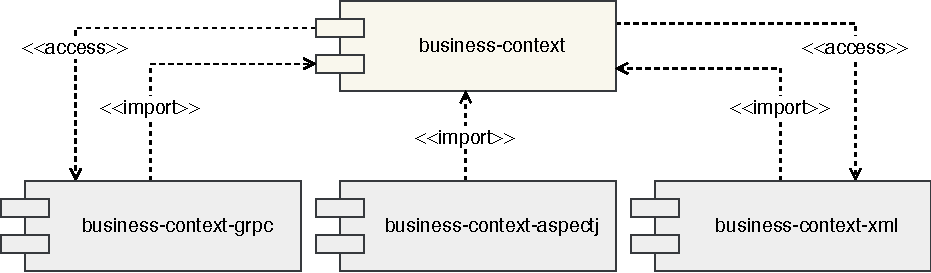
\includegraphics[keepaspectratio=true, width=1\linewidth]{figures/library-modules.pdf}
    \caption{Moduly prototypu knihovny pro jazyk Java a jejich závislosti}
    \label{fig:modules}
\end{figure}

\subsection{Správa závislostí projektu}

Pro správu závislost\'{\i} a automatickou kompilaci a sestavován\'{\i}
všech těchto modulů byl zvolen projekt \textit{Maven}\footnote{\url{https://maven.apache.org/}}.
Tento nástroj umožňuje v\'yvojáři komfortně a centrálně spravovat závislosti jeho projektu včetně
detailn\'{\i}ho popisu jejich verze. Dále také umožňuje specifikovat a rozšiřovat kompilaci projektu.

\subsection{Jádro knihovny}

% Jádro knihovny
Jádro knihovny obsahuje metamodel a registr byznysových kontextů, weaver byznysových pravidel
a logické výrazy pravidel. Registr kontextů implementuje třída \code{BusinessContextRegistry},
která kromě funkcí popsaných v sekci~\ref{sec:registry-design} umožňuje snadnou konfiguraci
stahování vzdálených byznysových kontextů a načítání lokálních kontextů z \gls{DSL} pomocí
návrhové vzoru Builder~\cite{fowler2002patterns}. Registr není závislý na konkrétních
technologiích použitých pro síťovou komunikaci ani na použitém \gls{DSL}.

% popis expressions
Logické výrazy byznysových pravidel jsou implementovány samostatnými třídami, které rozšiřují
jednotné rozhraní \code{Expression}. Toto rozhraní podporuje návrhový vzor Interpreter, který umožňuje
vyhodnocení výrazů, jak bylo popsáno v sekci~\ref{sec:expressions-design}. Zároveň je tím usnadněno
rozšíření knihovny o nové výrazy. Toto rozhraní navíc poskytuje metody, které usnadňují serializaci
výrazů.

\subsection{Weaving}

% popis weaveru
Weaver byznysových pravidel musí být schopen extrahovat informace o kontextu probíhající byznysové
operace, aby mohl správně zvolit příslušný byznysový kontext. V knihovne pro jazyk Java
byla pro tento účel zvolena anotace \code{BusinessOperation}, která umožňuje uživateli
knihovny označit metodu vykonávající byznysovou operaci. Parametry této metody mohou být
označeny anotací \code{BusinessContextParameter}. Weaver takto oanotované parametry vloží
jako proměnné do operačního kontextu a podmínky byznysových pravidel se na ně mohou odkazovat.
Ukázka použití těchto anotací je ve zdrojovém kódu~\ref{lst:business-operation-aspectj}.
Pomocí knihovny AspectJ\footnote{\url{https://www.eclipse.org/aspectj/}}, která poskytuje sadu nástrojů pro použití principů \gls{AOP},
je pak weaver pravidel volán ve chvíli, kdy je vykonávána anotovaná byznysová metoda.

\lstinputlisting[
caption={Označen\'{\i} operačn\'{\i}ho kontextu a jeho parametrů pomoc\'{\i} anotac\'{\i} Java knihovny},
label={lst:business-operation-aspectj},
language=Java,
%frame=single,
%float,
%floatplacement=H
]
{code/business_operation_aspectj.java}

\subsection{Serializace a deserializace XML}

% DSL XML
Pro serializaci a deserializici \gls{DSL} byznysových kontextů byly implementovány třídy
\code{BusinessContextXmlWriter} a \code{BusinessContextXmlLoader}. Ty využívají knihovnu
JDOM~2\footnote{\url{http://www.jdom.org/}}, která poskytuje
kompletn\'{\i} sadu nástroju pro čten\'{\i} a zápis \gls{XML} dokumentů.
Implementuje specifikaci \textit{Document Object Model}
pomoc\'{\i} které lze automaticky sestavovat a č\'{\i}st \gls{XML} dokumenty.

\subsection{Distribuce byznysových pravidel}

K distribuci byznysových pravidel mezi službami byly implementovány obsluhující třídy
\code{GrpcBusinessContextServer} a \code{GrpcBusinessContextClient}.
Framework gRPC poskytuje knihovnu pro jazyk Java, která vygeneruje \textit{Stub}
zapouzdřující veškerou síťovou komunikaci. Obsluha komunikace tak vyžaduje pouze
sepsání obslužného kódu, který převede byznysové kontexty z metamodelu a zpět.
Obě třídy navíc obsahují metody pro snadnou konfiguraci sítových adres.

\section{Knihovna pro platformu Python}

Knihovna pro platformu Python využ\'{\i}vá verzi jazyka 3.6, která byla v době
psaní práce nejnovější stabilní verzí. Knihovna se skládá ze tří částí: \code{business\_context} obsahuje jádro knihovny,
\code{business\_context\_grpc} umožňuje síťovou komunikaci pomocí frameworku
gRPC a \code{business\_context\_xml} poskytuje nástroje pro zápis a čtení kontextů z \gls{XML}.
Pomoc\'{\i} nástroje \textit{pip}\footnote{\url{https://pip.pypa.io/en/stable/}}
lze jednotlivé části knihovny nainstalovat a využ\'{\i}vat jako samostatné
Python moduly. Implementace odpov\'{\i}dá navržené specifikaci.

\subsection{Srovnán\'{\i} s knihovnou pro platformu Java}

\paragraph{Weaving} Největš\'{\i}m rozd\'{\i}lem oproti knihovně pro
jazyk Java je implementace weavingu byznys kontextů.
Jazyk Python totiž d\'{\i}ky své dynamické povaze a vestavěnému
systému dekorátorů umožňuje aplikovat principy aspektově orientovaného
programován\'{\i} bez potřeby dodatečn\'ych knihoven či technologi\'{\i}.
Zdrojov\'y kód~\ref{lst:python-weaving-example} znázorňuje
definici a použit\'{\i} dekorátoru \code{business\textunderscore operation}.
Dekorátoru je potřeba předat samotn\'y weaver, narozd\'{\i}l
od implementace v Javě, kdy se o předán\'{\i} weaveru postará dependency
injection container.

\lstinputlisting[
caption={Př\'{\i}klad použit\'{\i} dekorátorů pro weaving v jazyce Python},
label={lst:python-weaving-example},
language=Python,
%frame=single,
%float,
%floatplacement=H
]
{code/python_weaving.py}

\paragraph{Jména tříd a metod} Jazyk Python využívá jiné jmenné konvence
a jinak člení kód do jednotlivých souborů. Aby byly tyto konvence zachovány,
třídy knihovny a názvy jejich metod se liší od těch v jazyce Java.

\subsection{Použité technologie}

Jazyk Python poskytuje na rozdíl od jazyka Java téměř všechny nástroje, které byly pro implementaci
prototypu knihovny potřeba. Jedinou výjimkou byl modul pro obsluhu frameworku gRPC.
Ze standardní knihovny jazyka byly využity moduly \code{typing} pro statické typování,
\code{re} pro regulární výrazy, \code{enum} pro implementaci výčtových hodnot, \code{copy} pro
kopírování objektů, \code{fs} pro práci se soubory a \code{xml} pro práci s XML dokumenty.


\section{Knihovna pro platformu Node.js}

Knihovna pro platformu \textit{Node.js} byla implementována
v jazyce JavaScript, konkrétně ve verzi \textit{ECMAScript 6.0}.
Implementace odpov\'{\i}dá specifikaci návrhu, umožňuje
instalaci pomoc\'{\i} bal\'{\i}čkovac\'{\i}ho nástroje a snadnou
integraci do kódu v\'ysledné služby. Stejně jako knihovna
pro jazyk Python se skládá ze tří modulů: \code{business-context} obsahuje
jádro knihovny, \code{business-context-grpc} poskytuje server a klienta pro distribuci
byznysových kontextů po síti pomocí frameworku gRPC a \code{business-context-xml} umožňuje
serializaci a deserializaci z XML.

\subsection{Srovnán\'{\i} s knihovnou pro platformu Java}

\paragraph{Weaving} Podobně jako v knihovně pro jazyk Python,
i v knihovně pro Node.js byl oproti knihovně pro jazyk Java
největš\'{\i} rozd\'{\i}l v implementaci weavingu. Platforma Node.js
totiž nedisponuje žádnou kvalitn\'{\i} knihovnou, která by ulehčila
využit\'{\i} konceptů aspektově orientovaného programován\'{\i}.
Jazyk JavaScript však podobně jako jazyk Python umožňuje využ\'{\i}t
princip dekorátoru funkce. Ukázka takového dekorátoru je ve zdrojovém
kódu~\ref{lst:nodejs-weaving}. Funkce \code{register()} obsahuje logiku pro registraci uživatele,
která může obsahovat např\'{\i}klad uložen\'{\i} entity do databáze a odeslán\'{\i}
registračn\'{\i}ho emailu. Při exportován\'{\i} funkce z Node.js modulu
je využita funkce \code{wrapCall()}, která má za úkol dekorovat
předanou funkci \code{func}, před jej\'{\i}m zavolán\'{\i} vyhodnotit
preconditions a po zavolán\'{\i} aplikovat post-conditions.
D\'{\i}ky tomu bude každ\'y kód, kter\'y využije modul definuj\'{\i}c\'{\i} funkci
pro registraci uživatele, pracovat s dekorovanou funkc\'{\i}.

\paragraph{Využit\'{\i} gRPC} Narozd\'{\i}l od implementac\'{\i} knihovny
v jazyc\'{\i}ch Java a Python um\'{\i} knihovna obsluhuj\'{\i}c\'{\i} gRPC
fungovat i bez předgenerovaného kódu. To poněkud usnadnilo
práci při serializaci byznys kontextů do přenosového formátu
i při deserializaci a ukládán\'{\i} kontextů do paměti. Úspora
kódu je ale na úkor typové kontroly a tak může b\'yt kód náchylnějš\'{\i}
na lidskou chybu.

\lstinputlisting[
caption={Př\'{\i}klad dekorace funkce v JavaScriptu pro aplikaci weavingu},
label={lst:nodejs-weaving},
language=JavaScript,
%frame=single,
%float,
%floatplacement=H
]
{code/nodejs_weaving.js}

\subsection{Použité technologie}

%\goal{Použité technologie pro v\'yvoj knihovny}
Podobně jako byl použit nástroj Maven pro knihovnu v jazyce Java byl
využit bal\'{\i}čkovac\'{\i} nástroj \textit{NPM}, kter\'y je předinstalován
v běhovém prostřed\'{\i} \textit{Node.js}. Tento nástroj ale nedisponuje
př\'{\i}liš silnou podporou pro správu automatick\'ych sestaven\'{\i} knihovny
a v základn\'{\i}m nastaven\'{\i} nen\'{\i} ani př\'{\i}liš efektivn\'{\i} pro správu závislost\'{\i}.
Proto bylo nutné využ\'{\i}t dodatečné knihovny, jmenovitě
\textit{Yarn}\footnote{\url{https://yarnpkg.com/en/}}, \textit{Babel}\footnote{\url{https://babeljs.io/}} a
\textit{Rimraf}\footnote{\url{https://github.com/isaacs/rimraf}}.

\section{Systém pro centráln\'{\i} správu byznys pravidel}\label{sec:central-administration}

Součástí této práce je i implementace nástroje, který umožní centrální správu byznysových
pravidel. Ta vychází z návrhu popsaného v sekci~\ref{sec:central-administration-design}

\subsection{Popis implementace}

Systém pro centrální správu byl implementován jako webová služba v jazyce Java
s využitím frameworku Spring Boot\footnote{\url{https://projects.spring.io/spring-boot/}}.
Ten umožňuje využití návrhového vzoru Model-View-Controller, který je vhodný
pro aplikace s uživatelským rozhraním.

Model systému obsahuje třídu \code{BusinesssContextEditor}, která implementuje
návrhový vzor Facade~\cite{fowler2002patterns}. Umožňuje načtení byznysových
kontextů ze vzdálených služeb a jejich následnou úpravu a validaci. K tomu využívá
prototyp knihovny pro jazyk Java, díky kterému může kontexty přenášet po síti,
načítat a zapisovat ze do \gls{DSL} a využívat metamodel kontextů.

Pro komfortn\'{\i} obsluhu centráln\'{\i} administrace bylo naprogramováno
uživatelské rozhran\'{\i} pomoc\'{\i} technologi\'{\i} Hypertext Markup Language
(HTML) a Cascading Style Sheets (\gls{CSS}). V uživatelském rozhraní lze zobrazit
přehled všech byznysových kontextů a pomocí formulářů je upravovat a vytvářet nové.
Detail byznysového kontextu v uživatelském rozhran\'{\i} je zobrazen
na sn\'{\i}mku~\ref{fig:screenshot-context-detail} a formulář pro úpravu kontextu
na sn\'{\i}mku~\ref{fig:screenshot-context-edit}.

\subsection{Detekce a prevence potenciáln\'{\i}ch problémů}

%\goal{Problémy způsobené rozšiřován\'{\i}m kontextů}
Sekce~\ref{sec:context-inheritance} identifikuje problémy, které
mohou nastat při úpravě nebo vytvářen\'{\i} nového byznysového kontextu.
Kromě syntaktick\'ych chyb, které jsou detekovány automaticky pomoc\'{\i} definovaného schematu,
je potřeba detekovat následující sémantické chyby, které mohou b\'yt způsobeny rozšiřován\'{\i}m kontextů:
\begin{enumerate}[label=\alph*)]
    \item Neunikátní identifikátory byznysových pravidel
    \item Závislosti na neexistuj\'{\i}c\'{\i}ch kontextech
    \item Cyklus v grafu závislost\'{\i} kontextů
\end{enumerate}

%\goal{Chápán\'{\i} kontextů jako grafu}
Unikátnost byznysových pravidel lze zajistit postupným ukládáním jejich identifikátorů
do vhodné datové struktury a kontrolovat, zda v ní již nejsou obsaženy. Jako vhodná struktura
pro tento účel byl zvolen \code{Set}~\cite{hopcroft1983data}.
Kontexty a jejich vzájemné závislosti lze vn\'{\i}mat jako
orientovan\'y graf, kde uzel grafu reprezentuje kontext
a orientovaná hrana reprezentuje závislost mezi kontexty.
Směr závislosti lze pro tento účel zvolit libovolně.
Pro detekci závislosti na neexistuj\'{\i}c\'{\i}ch kontextech je nejprve
sestaven seznam existuj\'{\i}c\'{\i}ch kontextů a následně jsou navštíveny
jednotlivé hrany grafu kontextů a je ověřeno, zda existuj\'{\i} oba kontexty
nálež\'{\i}c\'{\i} dané hraně. Díky zvolen\'{\i} vhodn\'ych datov\'ych struktur
bylo dosaženo lineárn\'{\i} časové složitosti v závislosti na počtu hran grafu.
Pro detekci cyklů v grafu závislosti pravidel popsanou v sekci~\ref{sec:context-inheritance} byl
zvolen Tarjanův algoritmus~\cite{tarjan1971depth}. Ten umožňuje detekci souvisl\'ych
komponent a má lineárn\'{\i} složitost závislou na součtu počtu hran a
počtu uzlů grafu. V př\'{\i}padě, že zápis nového či upraveného kontextu obsahuje syntaktické
nebo sémantické chyby, administrace nedovol\'{\i} uživateli změnu provést a vyp\'{\i}še informativn\'{\i}
chybovou hlášku.

\section{Shrnutí}

%\goal{Dosáhli jsme vytyčen\'ych c\'{\i}lů implementace}
Na základě navrženého frameworku byly implementovány prototypy
knihoven pro platformy jazyka Java, jazyka Python a
Node.js. Knihovny umožňuj\'{\i} centráln\'{\i} správu a automatickou distribuci a integraci
byznysov\'ych kontextů, včetně vyhodnocován\'{\i} jejich pravidel, za
použit\'{\i} aspektově orientovaného př\'{\i}stupu.
V rámci této kapitoly byl specifikován \gls{DSL}, kter\'ym lze popsat
byznys kontext nezávisle na platformě.
Implementované protoypy knihoven lze využ\'{\i}t k implementaci služeb a k sestaven\'{\i}
funkčn\'{\i}ho systému, jak je popisáno v následuj\'{\i}c\'{\i} kapitole.

%\goal{Hostován\'{\i} na GitHubu + licence}
Vešker\'y kód implementace je hostován v centráln\'{\i}m repozitáři
ve službě GitHub\footnote{\url{https://github.com/klimesf/diploma-thesis}}
a je zpř\'{\i}stupněn pod open-source licenc\'{\i} \gls{MIT}~\footnote{\url{http://www.linfo.org/mitlicense.html}}.
Knihovny pro jednotlivé platformy tedy lze libovolně
využ\'{\i}vat, modifikovat a š\'{\i}řit.
